\documentclass[tikz,border=10pt]{standalone}
\usepackage{amsmath}
\usepackage{amssymb}
\definecolor{mantis}{RGB}{0, 105, 62}
\begin{document}
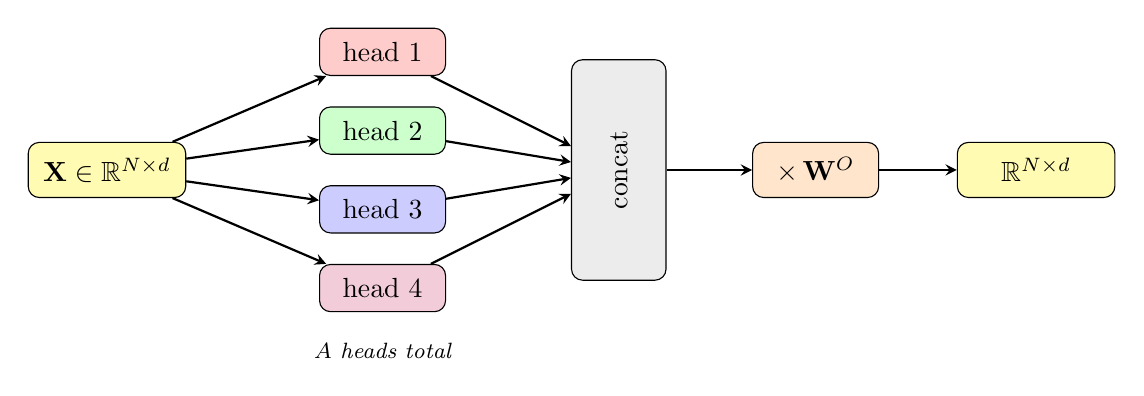
\begin{tikzpicture}[>=stealth]
    \node[draw, rounded corners, fill=yellow!30, minimum width=2cm, minimum height=0.7cm] (X) at (0,0) {$\mathbf{X} \in \mathbb{R}^{N \times d}$};
    \node[draw, rounded corners, fill=red!20, minimum width=1.6cm, minimum height=0.6cm] (h1) at (3.5,1.5) {head 1};
    \node[draw, rounded corners, fill=green!20, minimum width=1.6cm, minimum height=0.6cm] (h2) at (3.5,0.5) {head 2};
    \node[draw, rounded corners, fill=blue!20, minimum width=1.6cm, minimum height=0.6cm] (h3) at (3.5,-0.5) {head 3};
    \node[draw, rounded corners, fill=purple!20, minimum width=1.6cm, minimum height=0.6cm] (h4) at (3.5,-1.5) {head 4};
    \draw[->, thick] (X) -- (h1);  \draw[->, thick] (X) -- (h2);
    \draw[->, thick] (X) -- (h3);  \draw[->, thick] (X) -- (h4);
    \node[draw, rounded corners, fill=gray!15, minimum width=1.2cm, minimum height=2.8cm] (concat) at (6.5,0) {\rotatebox{90}{concat}};
    \draw[->, thick] (h1) -- (concat);  \draw[->, thick] (h2) -- (concat);
    \draw[->, thick] (h3) -- (concat);  \draw[->, thick] (h4) -- (concat);
    \node[draw, rounded corners, fill=orange!20, minimum width=1.6cm, minimum height=0.7cm] (WO) at (9,0) {$\times\,\mathbf{W}^O$};
    \draw[->, thick] (concat) -- (WO);
    \node[draw, rounded corners, fill=yellow!30, minimum width=2cm, minimum height=0.7cm] (out) at (11.8,0) {$\mathbb{R}^{N \times d}$};
    \draw[->, thick] (WO) -- (out);
    \node[font=\footnotesize\itshape] at (3.5,-2.3) {$A$ heads total};
\end{tikzpicture}
\end{document}
